% Preamble for: An Explicit Exponential-Period Representation of the V_quad Connection Coefficient
\documentclass[11pt,reqno]{amsart}
\usepackage[T1]{fontenc}
\usepackage{amsmath,amssymb,amsthm,mathtools}
\usepackage{microtype}
\usepackage[letterpaper,margin=1.5in]{geometry}
\usepackage{enumitem}
\usepackage{booktabs}
\usepackage{tikz}
\usetikzlibrary{arrows.meta,decorations.markings,decorations.pathmorphing}
\usepackage[colorlinks=true,linkcolor=blue,citecolor=blue,urlcolor=blue]{hyperref}

% --- byte-reproducible build guards (memory: reproducible PDFs) ---
\pdfinfoomitdate=1
\pdftrailerid{}
\pdfsuppressptexinfo=-1

% --- theorem environments ---
\theoremstyle{plain}
\newtheorem{theorem}{Theorem}[section]
\newtheorem{proposition}[theorem]{Proposition}
\newtheorem{lemma}[theorem]{Lemma}
\newtheorem{corollary}[theorem]{Corollary}
\theoremstyle{definition}
\newtheorem{definition}[theorem]{Definition}
\newtheorem{remark}[theorem]{Remark}
\newtheorem{example}[theorem]{Example}

% --- macros ---
\newcommand{\Vquad}{V_{\mathrm{quad}}}
\newcommand{\Bhat}{\widehat{B}}
\newcommand{\Lphi}{L_{\varphi}}
\newcommand{\LV}{L_{V}}
\newcommand{\Qsqrt}{\mathbb{Q}(\sqrt3)}
\newcommand{\Qbar}{\overline{\mathbb{Q}}}
\newcommand{\xizero}{\xi_0}
\newcommand{\SL}{\mathrm{SL}}
\newcommand{\GL}{\mathrm{GL}}
\newcommand{\Gm}{\mathbb{G}_m}
\providecommand{\C}{}\renewcommand{\C}{C}
\DeclareMathOperator*{\K}{K}

\title[An exponential-period representation of the $V_{\mathrm{quad}}$ constant]%
{An explicit exponential-period representation of the $V_{\mathrm{quad}}$ connection coefficient}
\author{Papanokechi}
\thanks{ORCID \texttt{0009-0000-6192-8273}. This is a working draft; not yet submitted.}
\date{15 June 2026}

\begin{document}
\begin{abstract}
We prove that the connection coefficient $C$ of the $\Vquad$ polynomial continued fraction---the
rank-one standalone closure on the Sakai surface $D_5^{(1)}$ (Painlev\'e~V)---admits an explicit
exponential-period representation
$C=(\lvert\Gamma(\beta)\rvert/2\pi)\int_\gamma e^{\xi}\Bhat(\xi)\,d\xi=\lvert\Gamma(\beta)\rvert K$,
where $\Bhat$ is the Borel transform of the $\Vquad$ asymptotic series, holonomic of order $4$
with coefficients in the real quadratic field $\Qsqrt$; $\gamma$ is an explicit Hankel
rapid-decay cycle on $(-\infty,-2/\sqrt3]$; and $\beta=-1/(3\sqrt3)$. The identity is verified by
three structurally independent methods---differential-equation/operator duality, Borel--Laplace
contour deformation, and Stokes-data---agreeing to $46$ digits. The order-$2$ operator annihilating
the asymptotic series has differential Galois group $\SL_2(\mathbb{C})$ by Kovacic's algorithm.
As a by-product, holonomicity of the Borel transform forces a finite resurgent structure. Finally,
conditional on the Fres\'an--Jossen period conjecture for exponential motives and on a stated
motivic-comparison hypothesis, $C$ is transcendental over $\Qbar$.
\end{abstract}
\maketitle

% ===== section-1.md =====
\section{Introduction}\label{sec:intro}

\subsection{The V\_quad continued fraction and its connection coefficient}
Let $\Vquad$ denote the polynomial continued fraction
\begin{equation}\label{eq:vquad-pcf}
  \Vquad \;=\; 1 \;+\; \K_{n\ge 1}\,\frac{1}{\,3n^{2}+n+1\,}
  \;=\; 1+\cfrac{1}{\,5+\cfrac{1}{\,15+\cfrac{1}{\,31+\cdots}}}\,,
\end{equation}
the partial denominators being the quadratic $b_n=3n^2+n+1$ and all partial numerators $1$.
This is the rank-one ($n=1$) standalone member of the V\_quad family studied in the V\_quad
companion paper~\cite{Vquad}, where it is identified as a non-classical Painlev\'e~V
transcendent on the Sakai surface $D_5^{(1)}$ (symmetry $W(A_3^{(1)})$, $\delta=-\tfrac12\ne0$,
in the surface/symmetry classification of~\cite{SakaiClass}),
with formal monodromy exponent $\theta_\infty=2/\sqrt3$ and $\alpha=\theta_\infty^2/8=\tfrac16$.
The asymptotic (WKB/Riccati) solution of the associated problem is a Gevrey-1 formal power
series
\begin{equation}\label{eq:phi-series}
  \varphi(z)\;=\;\sum_{n\ge 0} a_n z^n ,\qquad a_0=1,
\end{equation}
whose Borel transform has an isolated singularity at the \emph{action}
$\xizero=2/\sqrt3=1.15470053837925\ldots$ of branch type governed by the exponent
\begin{equation}\label{eq:beta}
  \beta=-\frac{1}{3\sqrt3}=-0.19245008972987525\ldots
\end{equation}
The \emph{connection coefficient} $\C$ of $\Vquad$ is the Borel branch amplitude attached to
that singularity; in the standard resurgence normalisation~\cite{Dingle,BerryHowls,StokesNote}
it equals
\begin{equation}\label{eq:C-skeleton}
  \C \;=\; \lvert\Gamma(\beta)\rvert\cdot K,\qquad
  K=0.0728781025518669641294\ldots,
\end{equation}
where $K$ is the prefactor-stripped Dingle late-term amplitude of~\eqref{eq:phi-series}. The
companion Stokes constant is $S=2\pi K=0.4579066231690176361190\ldots$, and the two normalisations
are tied by the exact bridge identity
\begin{equation}\label{eq:bridge}
  \frac{S}{\C}\;=\;\frac{2\pi}{\lvert\Gamma(\beta)\rvert}\qquad(\text{residual }0).
\end{equation}
The constant $\C$ governs the inter-sectorial (Stokes) jump of the Borel sum of $\varphi$ and is,
in the language of the parent program, the arithmetic fingerprint of the $\Vquad$ transcendent.

\subsection{The Sakai-stratification context}
The present paper is a self-contained contribution to one entry of a larger program, the
\emph{Sakai stratification of polynomial-continued-fraction transcendence}~\cite{Sakai}, which
classifies PCF limits by the Sakai surface type of the Painlev\'e isomonodromy governing their
tails and asks, for each stratum, whether the associated connection constant admits a period
interpretation. For the $D_5^{(1)}$ (Painlev\'e~V) stratum the master conjecture predicts that
$\C$ is an \emph{exponential period} in the sense of Fres\'an--Jossen~\cite{FJ}; the entry was
previously graded \emph{structural} (the skeleton $\Gamma(\beta)\cdot K$ matches, but no explicit
period integral was exhibited). All objects used below are defined in-paper, so no familiarity
with~\cite{Sakai} is required.

The significance is not confined to the program. Exhibiting a specific, independently interesting
constant as an explicit exponential period---rather than merely asserting it should be one---is the
kind of evidence the Kontsevich--Zagier and Grothendieck period philosophies call for: the
arithmetic of a number is conjecturally governed by the geometry of a motive realising it as a
period, and concrete realisations are scarce, especially for \emph{divergent}-series (Stokes)
constants rather than convergent integrals. The constant $\C$ here arises from a continued fraction
of the type produced en masse by the Ramanujan Machine~\cite{RamanujanMachine}, so the method also
indicates how the transcendence of machine-discovered constants might be approached structurally
rather than case by case.

\subsection{Main results}
We exhibit $\C$ as an explicit exponential-period integral and verify the identity three
independent ways. Write $\Bhat(\xi)=\sum_{m\ge0}b_m\xi^m$, $b_m=a_{m+1}/m!$, for the Borel
transform of~\eqref{eq:phi-series}, and let $\gamma$ be the Hankel thimble wrapping the cut
$(-\infty,-\xizero]$ (Definition~\ref{def:gamma}).

\begin{theorem}[Explicit exponential-period representation]\label{thm:main}
The Borel transform $\Bhat$ is holonomic with coefficients in the real quadratic field
$\Qsqrt$, annihilated by an explicit order-$4$ operator $\LV$ (Theorem~\ref{thm:LV}); the
cycle $\gamma$ is a rapid-decay cycle for the potential $f=-\xi$
(Proposition~\ref{prop:rapiddecay}); and
\begin{equation}\label{eq:main-identity}
  \boxed{\;\C\;=\;\frac{\lvert\Gamma(\beta)\rvert}{2\pi}\int_{\gamma} e^{\xi}\,\Bhat(\xi)\,d\xi
  \;=\;\lvert\Gamma(\beta)\rvert\cdot K\;}
\end{equation}
where the raw thimble integral equals $S\,e^{-\xizero}$ at leading order and $\C$ is recovered
by the explicit algebraic-$\Gamma$ factor $\lvert\Gamma(\beta)\rvert/2\pi$. The identity is
verified by three structurally independent methods---differential-equation/operator duality,
Borel--Laplace/Hankel, and Stokes-data---which agree to $46$ significant digits
(Section~\ref{sec:verif}).
\end{theorem}

The differential input is sharp. The series $\varphi$ is $D$-finite over \emph{exactly} $\Qsqrt$
(minimal operator $\Lphi$ of order $2$, degree $4$), and its differential Galois group is as
large as possible.

\begin{theorem}[Galois group of $\Lphi$]\label{thm:galois}
The differential Galois group of $\Lphi$ over $\Qsqrt(z)$ is $\SL_2(\mathbb{C})$. This is proved
twice: by Kovacic case-elimination and by a structural torus-plus-unipotent argument
(Section~\ref{sec:operators}, certificate in Appendix~\ref{app:kovacic}).
\end{theorem}

Holonomicity of $\Bhat$ has an immediate qualitative consequence for the resurgence of $\Vquad$.

\begin{corollary}[Finite resurgence]\label{cor:finite}
Because $\Bhat$ is holonomic of order $4$, it has only finitely many singularities, namely
$\{0,-\xizero,\infty\}$. In particular there is \emph{no} infinite alien tower at
$2\xizero,3\xizero,\dots$: the resurgent structure of $\Vquad$ is a finite rank-$4$ connection,
not a wild lattice (Section~\ref{sec:operators}).
\end{corollary}

Finally, interpreting~\eqref{eq:main-identity} in the Fres\'an--Jossen framework yields a
conditional transcendence statement. We are careful to flag \emph{both} layers of
conditionality.

\begin{corollary}[Conditional transcendence]\label{cor:transc}
Assume \emph{(i)} the Fres\'an--Jossen period conjecture for exponential motives
\textup{(\cite{FJ}, Conjecture~1.3.2)}, and \emph{(ii)} that the de Rham realisation computed
here represents the motivic Galois group of the exponential motive
$M=(\mathbb{A}^1\smallsetminus\{0,-\xizero\},\,f=-\xi,\,\Bhat\,d\xi)$ \textup{(the comparison
gap G-MOTGALOIS, Section~\ref{sec:fj})}. Then the V\_quad connection coefficient $\C$ is
transcendental over $\Qbar$.
\end{corollary}

\subsection{What is and is not computer-algebra-automatable here}
The differential backbone of this paper is squarely within reach of present-day symbolic
software, and we have used it: the recognition of $\Lphi$ and $\LV$ from the coefficient stream
is exactly holonomic guessing as implemented in \texttt{gfun}~\cite{gfun} and
\texttt{ore\_algebra}~\cite{oreAlgebra}; the Kovacic decision and the differential-Galois data
are the province of Kovacic's algorithm~\cite{Kovacic} and of packages such as Maple's
\texttt{DEtools[DifferentialGaloisGroup]} (we reproduced the Kovacic verdict by case-elimination
and by an independent structural argument, Appendix~\ref{app:kovacic}); and the Borel--Pad\'e
and large-order extractions are standard exponential-asymptotics computations. What is
\emph{not} automatable, and what constitutes the mathematical content of the paper, is
(a)~the identification of the precise rapid-decay cycle $\gamma$ and the proof that the three
period-extraction routes agree, and (b)~the motivic interpretation
(Corollary~\ref{cor:transc}), which lies beyond any current CAS. We return to this comparison
in Section~\ref{sec:disc} and Appendix~\ref{app:repro}.

\subsection{Organisation}
Section~\ref{sec:operators} constructs and verifies $\Lphi$ and $\LV$, proves
Theorem~\ref{thm:galois} and Corollary~\ref{cor:finite}. Section~\ref{sec:cycle} defines the
cycle $\gamma$ and establishes its rapid-decay property and Fres\'an--Jossen compatibility.
Section~\ref{sec:main} states and normalises the main identity. Section~\ref{sec:verif} gives
the three verifications and their cross-check. Section~\ref{sec:fj} applies the
Fres\'an--Jossen framework and proves Corollary~\ref{cor:transc}.
Section~\ref{sec:disc} discusses the place of the result in the stratification program, the
$d\ge3$ obstruction, and the relation to the Ramanujan-Machine/conservative-matrix-field
circle of ideas. Appendices collect the explicit coefficients, the Kovacic certificate, the
numerical logs, the four sign-convention enumeration for the differential-equation method, and
the reproducibility statement.

\subsection{Notation and conventions}
Throughout, $\Qsqrt=\mathbb{Q}(\sqrt3)$ is the real quadratic field generated by the V\_quad
Riccati seed $\sigma=-1/\sqrt3$, and $\Qbar$ the algebraic closure of $\mathbb{Q}$. We write
$D_z=d/dz$ and $D_\xi=d/d\xi$ (abbreviated $D$ when the variable is clear), and treat differential
operators as elements of the Weyl algebra $\Qsqrt\langle z,D_z\rangle$ (resp.\ in $\xi$). The
\emph{order} of an operator is its degree in $D$ and its \emph{degree} is the maximal polynomial
degree of its coefficients. The Borel transform is taken at Gevrey order $1$, $b_m=a_{m+1}/m!$,
mapping the divergent series $\varphi(z)=\sum a_nz^n$ to the convergent germ
$\Bhat(\xi)=\sum b_m\xi^m$; the dual variables satisfy $z\leftrightarrow1/\xi$ at the level of
exponential scales, with the operator intertwiner~\eqref{eq:duality}. The action is
$\xizero=2/\sqrt3$, the branch exponent $\beta=-1/(3\sqrt3)$, and we use the resurgence
normalisation in which the Stokes constant is $S=2\pi K$ with $K$ the prefactor-stripped Dingle
amplitude. The potential is written $f=-\xi$ in the task convention, equal to $-f_{\mathrm{FJ}}$ in
the Fres\'an--Jossen sign convention (Remark~\ref{rmk:fjsign}); the period pairing is
$\langle e^{-f}\omega,\gamma\rangle=\int_\gamma e^{\xi}\Bhat(\xi)\,d\xi$. All numerical constants
are reported to the precision at which they were certified (typically $46$--$58$ digits);
``residual $0$'' means an exact identity in $\Qsqrt$, while a residual such as
$8.84\times10^{-46}$ is a high-precision floating check.

% ===== section-2.md =====
\section{The differential operators \texorpdfstring{$\Lphi$}{Lphi} and \texorpdfstring{$\LV$}{LV}}\label{sec:operators}

Throughout, $D=d/dz$ on the $\varphi$-side and $D=d/d\xi$ on the Borel side; the base field is
the real quadratic number field $\Qsqrt$. Every coefficient below is exact in $\Qsqrt$, obtained
by linear algebra over $\Qsqrt$ (Fraction pairs $p+q\sqrt3$), \emph{not} by numerical
integer-relation search; the annihilation residuals are identically zero in $\Qsqrt$, not merely
small. Full coefficient listings and the verification protocol are in
Appendix~\ref{app:coeffs}.

The exactness is concrete already at the level of the coefficient stream. Seeding the V\_quad
Riccati recursion with $\sigma=-1/\sqrt3$ (so $\sigma^2=\tfrac13\in\mathbb{Q}$,
$1/\sigma=-\sqrt3$) produces every $a_n$ as an exact element $p+q\sqrt3$ of $\Qsqrt$; the first
few, and the corresponding Borel coefficients $b_m=a_{m+1}/m!$, are
(script \texttt{holonomic\_recognition\_q3.py}, \texttt{PERIOD-REP-VQUAD-002}):
\begin{equation}\label{eq:coeffstream}
\renewcommand{\arraystretch}{1.25}
\begin{array}{r|l|l}
 n & a_n\in\Qsqrt & \text{(decimal)}\\\hline
 0 & 1 & 1.0000000000\\
 1 & -\tfrac{1}{12}-\tfrac{1}{24}\sqrt3 & -0.1555021170\\
 2 & -\tfrac{73}{1152}-\tfrac{17}{648}\sqrt3 & -0.1088076601\\
 3 & \tfrac{6589}{41472}-\tfrac{13415}{746496}\sqrt3 & \phantom{-}0.1277522430\\
 4 & \tfrac{9247897}{71663616}-\tfrac{846407}{4478976}\sqrt3 & -0.1982654887
\end{array}
\end{equation}
with e.g.\ $b_0=a_1$, $b_1=a_2$, $b_2=\tfrac{6589}{82944}-\tfrac{13415}{1492992}\sqrt3=
0.0638761215\ldots$. The exactness of these rationals is what licenses the word ``provably'' in
all field claims below: no step uses a numerical approximation of $\sqrt3$.

\subsection{The operator \texorpdfstring{$\Lphi$}{Lphi}}
\begin{theorem}[$\varphi$ is $D$-finite over $\Qsqrt$]\label{thm:Lphi}
The series $\varphi(z)=\sum_{n\ge0}a_nz^n$ of~\eqref{eq:phi-series} is annihilated by a unique
minimal operator
\[
  \Lphi \;=\; q_2(z)\,D^2 + q_1(z)\,D + q_0(z),\qquad q_i\in\Qsqrt[z],
\]
of order $2$ and degree $4$, with
\begin{align*}
  q_0(z)&=1+\Bigl(\tfrac{23}{9}+\tfrac{14}{27}\sqrt3\Bigr)z
              +\Bigl(-\tfrac{253}{9}+\tfrac{488}{27}\sqrt3\Bigr)z^2,\\
  q_1(z)&=(48-24\sqrt3)+(-64+44\sqrt3)z+\Bigl(-\tfrac{68}{3}+\tfrac{52}{3}\sqrt3\Bigr)z^2
              +\Bigl(-\tfrac{152}{3}+\tfrac{100}{3}\sqrt3\Bigr)z^3,\\
  q_2(z)&=(-36+24\sqrt3)z^2+(-12+8\sqrt3)z^3+(-12+8\sqrt3)z^4
           \;=\;4(2\sqrt3-3)\,z^2\,(z^2+z+3).
\end{align*}
The annihilation $\Lphi\varphi=0$ holds exactly in $\Qsqrt$ for every power $z^0,\dots,z^{139}$
tested; the minimal $(\text{order},\text{degree})$ has nullity $1$, and the higher nullities
$\{1,3,5,7\}$ (order $2$) and $\{2,6,10,14\}$ (order $3$) match the left-multiple count
$d-4+1$ of a single minimal order-$2$ operator, so there are no spurious solutions.
\end{theorem}

The coefficient field is \emph{exactly} $\Qsqrt$: all computations close over $\Qsqrt$, and both
$q_1,q_0$ carry genuine $\sqrt3$ parts, so the field is neither smaller (not $\mathbb{Q}$) nor
larger. Operationally $\Lphi$ is the scalar (Schr\"odinger) reduction of the V\_quad Painlev\'e-V
linear problem, recovered from the Riccati linearisation $c=\psi'/\psi$; the parent corpus
records the existence of this linear problem only verbally~\cite{Vquad}, and Theorem~\ref{thm:Lphi}
makes it explicit.

\begin{remark}[Provenance of $\Lphi$]\label{rmk:provenance}
We stress that $\Lphi$ is obtained by holonomic recognition from the coefficient stream
$(a_n)$---guessing an annihilating operator and then certifying $\Lphi\varphi=0$ exactly over
$\Qsqrt$---and \emph{not} from an a~priori Lax pair. The literature provides no explicit classical
Lax pair for the $\Vquad$ transcendent (a dedicated search returned none;
\texttt{PERIOD-REP-VQUAD-002}, \texttt{lax-pair-found.md}), so the holonomic route is the available
one and is in fact stronger here: it yields the minimal operator with a verifiable exact
certificate rather than a gauge-dependent matrix. The two exponential parts
$\exp(\pm(1/\sqrt3)/z)$ at $z=0$ found below are consistent with the V\_quad WKB/Riccati seed
$\sigma=-1/\sqrt3$ ($\sigma^2=1/3\in\mathbb{Q}$) and with the formal monodromy exponent
$\theta_\infty=2/\sqrt3$ of~\cite{Vquad}.
\end{remark}

\subsection{Singular structure of \texorpdfstring{$\Lphi$}{Lphi} and its Galois group}
Reducing $\Lphi$ to normal form $u''=r\,u$ via $y=u\exp(-\tfrac12\int q_1/q_2)$ gives, with
$a=q_1/q_2$, $b=q_0/q_2$ and $r=\tfrac14a^2+\tfrac12a'-b$,
\begin{equation}\label{eq:r}
  r(z)\;=\;\frac{11z^4+4z^2+4z+12}{\,4\,z^4\,(z^2+z+3)^2\,}.
\end{equation}
The poles of $r$ are $z=0$ (order $4$), the two roots $z=\tfrac{-1\pm i\sqrt{11}}2$ of $z^2+z+3$
(order $2$ each), and $o(\infty)=4$; the leading Laurent coefficient at $z=0$ is
$r\sim\tfrac13 z^{-4}$. Thus $z=0$ is an irregular singular point of Poincar\'e rank $1$ with two
distinct exponential parts $\exp(\pm(1/\sqrt3)/z)$; the two finite poles $\rho_\pm$ are
regular-singular for the reduced equation, and the point at infinity is regular-singular with
exponent difference fixed by $o(\infty)=4$. Only the irregular point $z=0$ carries the Stokes
phenomenon, and it is there that the connection coefficient lives. Table~\ref{tab:config}
summarises the singular configuration of $\Lphi$ alongside its Borel dual $\LV$.

\begin{table}[h]
\centering
\begin{tabular}{@{}lll@{}}
\toprule
 & $\Lphi$ (order $2$, on $z$) & $\LV$ (order $4$, on $\xi$) \\
\midrule
order / degree & $2$ / $4$ & $4$ / $2$ \\
base field & $\Qsqrt$ & $\Qsqrt$ \\
finite singularities & $\rho_\pm=\tfrac{-1\pm i\sqrt{11}}2$ (reg.) & $0$ (apparent), $-\xizero$ (branch) \\
irregular point & $z=0$, Poincar\'e rank $1$ & $\xi=\infty$, slope $1$ \\
Stokes datum & $S=2\pi K$ at $z=0$ & branch amplitude $A$ at $-\xizero$ \\
Galois group & $\SL_2(\mathbb{C})$ (Thm.~\ref{thm:galois}) & $G_V\supseteq\Gm\times(\SL_2\text{-dual})$ \\
\bottomrule
\end{tabular}
\caption{Singular configuration of the $\varphi$-side operator $\Lphi$ and its Borel dual $\LV$.
The irregular point of $\Lphi$ (at $z=0$) and the branch of $\LV$ (at $-\xizero$) are the two
faces of the same connection datum under Borel--Laplace duality. Source:
\texttt{PERIOD-REP-VQUAD-002}, \texttt{operator-verification.md} \S4.}
\label{tab:config}
\end{table}

\begin{proof}[Proof of Theorem~\ref{thm:galois}]
We give both arguments.

\emph{(1) Kovacic case-elimination.} In the Kovacic case/group
dictionary~\cite{Kovacic,vdPS} for $u''=ru$: Case~3 (finite groups $A_4,S_4,A_5$) requires every
pole order $\le2$; the pole of order $4$ at $z=0$ excludes it. Case~1 (reducible, $G\subseteq$
Borel) holds iff the Riccati equation $v'=r-v^2$ has a rational solution; a complete rational
Riccati solver returns none. Case~2 (imprimitive, $G\subseteq N(T)$) holds, given Case~1
excluded, iff the symmetric square $\Lphi^{\odot2}=D^3-4rD-2r'$ has a rational solution; the
ansatz $f=N(z)/\bigl(z^8(z^2+z+3)^4\bigr)$, $\deg N\le18$, yields a homogeneous linear system in
$38$ rational unknowns whose only solution is trivial. With Cases~1,2,3 excluded, the algorithm
returns Case~4: $G=\SL_2(\mathbb{C})$.

\emph{(2) Structural argument.} The reduced equation $u''=ru$ has no first-order term, so the
Wronskian is constant and $G\subseteq\SL_2$. At $z=0$ the two distinct exponentials
$\exp(\pm(1/\sqrt3)/z)$ generate the full diagonal torus $\mathbb{G}_m\subset\SL_2$ (the local
exponential torus). The nonvanishing Stokes constant $S=2\pi K\ne0$ at this irregular point is a
nonidentity unipotent off that torus. A maximal torus together with one off-torus unipotent
generate $\SL_2$, whence $G=\SL_2(\mathbb{C})$.
\end{proof}

The two routes are genuinely independent---an exhaustive negative search versus a positive
generation argument from the Stokes datum---and agree. (Only one symbolic engine was available;
the second route supplies the cross-check that a second computer-algebra system would otherwise
provide. See Appendix~\ref{app:kovacic}.)

\subsection{The Borel operator \texorpdfstring{$\LV$}{LV}}
We construct $\LV$ from $\Lphi$ by Borel--Laplace duality. The (formal) Borel transform of order
$1$ acts on the coefficient stream by $a_{m+1}\mapsto b_m=a_{m+1}/m!$; equivalently, on series, it
is the Hadamard-type rescaling that turns the Gevrey-$1$ divergent $\varphi$ into the convergent
germ $\Bhat$. On operators it intertwines the two differential structures by
\begin{equation}\label{eq:formalduality}
  z^2 D_z\ \longleftrightarrow\ \xi,\qquad \tfrac1z\ \longleftrightarrow\ D_\xi,
\end{equation}
the same intertwiner~\eqref{eq:duality} used analytically in Section~\ref{sec:verif}. Under it a
term $z^{a}D_z^{k}$ of $\Lphi$ maps to a term of $\xi$-degree bounded by the original
$z$-\emph{order} and of $\xi$-order bounded by the original $z$-\emph{degree}: order and degree are
exchanged. Hence the order-$2$, degree-$4$ operator $\Lphi$ produces an operator of order $4$ and
degree $2$ in $\xi$, and $D$-finiteness is preserved because~\eqref{eq:formalduality} is an
isomorphism of the Weyl algebra $\Qsqrt\langle\xi,D_\xi\rangle$. We verify the resulting operator
directly on the coefficient stream rather than relying on the formal map alone.

\begin{theorem}[$\Bhat$ is holonomic over $\Qsqrt$]\label{thm:LV}
The Borel transform $\Bhat(\xi)=\sum_{m\ge0}b_m\xi^m$, $b_m=a_{m+1}/m!$, is annihilated by a
unique minimal operator $\LV=\sum_{k=0}^4 p_k(\xi)D^k$ of order $4$ and degree $2$, normalised by
$p_0\equiv1$, with $p_1,\dots,p_4\in\Qsqrt[\xi]$ given explicitly in
Appendix~\ref{app:coeffs}. The residual $\LV\Bhat$ is identically zero in $\Qsqrt$ for every power
$\xi^0,\dots,\xi^{129}$ tested. The leading coefficient factors exactly as
\begin{equation}\label{eq:p4-factor}
  p_4(\xi)\;=\;\frac{210276+9720\sqrt3}{418501}\;\xi\,\Bigl(\xi+\frac{2}{\sqrt3}\Bigr),
  \qquad 418501=431\times971,
\end{equation}
so the singular locus of $\LV$ is $\{0,\,-\xizero=-2/\sqrt3,\,\infty\}$.
\end{theorem}

\begin{proposition}[Local exponents]\label{prop:exponents}
The local exponents of $\LV$ are
\[
  \{-1,0,1,2\}\ \text{at } \xi=0,\qquad
  \{\,-(1+\beta),\,0,1,2\,\}\ \text{at } \xi=-\xizero,\qquad
  \text{irregular of slope }1\ \text{at } \xi=\infty,
\]
with $-(1+\beta)=-1+\sqrt3/9=-0.80754991027\ldots$ the unique non-integer exponent. At $\xi=0$
the four exponents are consecutive integers, so the point is \emph{apparent} (single-valued, $\Bhat$
itself is the holomorphic exponent-$0$ solution). At $\xi=-\xizero$ the branch is carried by the
single irrational exponent $-(1+\beta)$, governing $\Bhat(\xi)\sim A\,(\xi+\xizero)^{-(1+\beta)}$
and hence the large-order law $a_n\sim \Gamma(n+\beta)/\xizero^{\,n+\beta}$ up to the amplitude
$A$. Both statements are obtained twice, by a falling-factorial indicial computation and by direct
solution of the Frobenius recurrence at $-\xizero$ (residuals $1.6\times10^{-46}$, no
logarithms); see Appendix~\ref{app:numlogs}.
\end{proposition}

\begin{remark}[From branch exponent to large-order law]\label{rmk:largeorder}
The single irrational exponent at $-\xizero$ controls the divergence of $\varphi$. Writing the
branch as $\Bhat(\xi)\sim A(\xi+\xizero)^{-(1+\beta)}$ and inverting the Borel transform
$b_m=a_{m+1}/m!$ term by term against $(\xi+\xizero)^{-(1+\beta)}=\xizero^{-(1+\beta)}\sum_m
\binom{-(1+\beta)}{m}(\xi/\xizero)^m$ gives, by Stirling,
\begin{equation}\label{eq:largeorder}
  a_n\;\sim\;\frac{S}{2\pi i}\,\frac{\Gamma(n+\beta)}{\xizero^{\,n+\beta}}\qquad(n\to\infty),
\end{equation}
the standard resurgence late-term law with action $\xizero=2/\sqrt3$ and characteristic exponent
$\beta=-1/(3\sqrt3)$. Thus the operator datum at $-\xizero$ (an algebraic exponent in $\Qsqrt$)
and the analytic datum $K$ governing $\lvert a_n\rvert$ are two readings of the same branch; the
amplitude $\lvert A\rvert=K\,\Gamma(1+\beta)$ relates them (Section~\ref{sec:verif}).
\end{remark}

\begin{remark}[Sign of the action]
The dominant Borel singularity lies on the \emph{negative} real axis at $-\xizero$. The modulus
$\xizero=2/\sqrt3$ was known to $95.6$ digits from $\lim_n\lvert a_n/a_{n+1}\rvert\,n$, but as a
modulus the sign was unpinned; the exact factorisation~\eqref{eq:p4-factor} fixes it, consistently
with $a_n\sim(-1)^{n+1}\lvert a_n\rvert$ for $n\ge3$, i.e. $b_m\sim(-1)^m(+)$. This places the cut
in the direction $\arg\xi=\pi$, which is exactly the rapid-decay direction for $f=-\xi$
(Section~\ref{sec:cycle}).
\end{remark}

\subsection{Finite resurgence}
\begin{proof}[Proof of Corollary~\ref{cor:finite}]
A holonomic function has finitely many singularities, located among the zeros of the leading
coefficient of its annihilator and the point at infinity. By Theorem~\ref{thm:LV} the leading
coefficient $p_4$ vanishes only at $0$ and $-\xizero$, so
$\operatorname{Sing}(\Bhat)\subseteq\{0,-\xizero,\infty\}$; the point $0$ is apparent
(Proposition~\ref{prop:exponents}), leaving the genuine singularities $-\xizero$ and the
irregular $\infty$. In particular $\Bhat$ has no singularity at $2\xizero,3\xizero,\dots$, so the
hypothetical infinite alien tower (in the sense of \'Ecalle's alien calculus~\cite{Ecalle})
suggested by the $(1/2)^n$ numerical floor in the parent probe
does not exist; the resurgence of $\Vquad$ is governed by the finite rank-$4$ connection $\LV$.
\end{proof}

This finiteness is what makes the period analysis of Section~\ref{sec:verif} possible at all: a
single branch at $-\xizero$ carries the entire connection datum, and the thimble of
Section~\ref{sec:cycle} sees exactly that branch.

\begin{lemma}[The apparent point carries no period]\label{lem:apparent}
The singularity of $\Bhat$ at $\xi=0$ contributes nothing to any rapid-decay period: its local
exponents $\{-1,0,1,2\}$ are consecutive integers, so the local monodromy is trivial and $\Bhat$
extends holomorphically across $0$ (it is the exponent-$0$ solution). Hence no cut emanates from
$0$, and the only branch a thimble can wrap is the one at $-\xizero$.
\end{lemma}

\begin{proof}
At a regular-singular point with integer exponents differing by integers and no logarithmic
solution, the local solution space contains a single-valued generator for each exponent, with the
top exponent solution holomorphic; the indicial data at $0$
(\eqref{eq:p4-factor} gives a simple zero of $p_4$ at $0$, and the falling-factorial indicial
polynomial $\propto s(s-2)(s-1)(s+1)$ has roots $\{-1,0,1,2\}$) shows $\Bhat$, the exponent-$0$
member, is holomorphic. Triviality of the monodromy is the definition of an apparent singularity.
Source: \texttt{PERIOD-REP-VQUAD-002}, \texttt{operator-verification.md}~\S4.2.
\end{proof}

\subsection{Algebraicity for Fres\'an--Jossen}
Theorems~\ref{thm:Lphi} and~\ref{thm:LV} discharge the load-bearing Fres\'an--Jossen axiom for
the eventual motive: $\omega=\Bhat(\xi)\,d\xi$ is an algebraic de Rham form for the twisted
connection $E^{-f}\otimes(\mathcal{O}^4,\nabla_{\LV})$ with $f=-\xi$, defined over the number
field $\Qsqrt$. The transcendental Painlev\'e-V accessory parameter of $\Vquad$ lives in the
\emph{nonlinear} moduli; the \emph{linear} scalar reduction governing the asymptotics is over
$\Qsqrt$, which is why no transcendental constant enters $\Lphi$ or $\LV$. We make the motivic
use of this precise in Section~\ref{sec:fj}.

% ===== section-3.md =====
\section{The rapid-decay cycle \texorpdfstring{$\gamma$}{gamma}}\label{sec:cycle}

This section makes the cycle $\gamma$ of Theorem~\ref{thm:main} precise, verifies that it is a
rapid-decay cycle in the Fres\'an--Jossen sense, and records its relative-homology class. All
statements are sourced to the probe deliverables
\texttt{cycle-formal-definition.md} and \texttt{rapid-decay-verification.md} of the slot
\texttt{PERIOD-REP-VQUAD-003}.

\subsection{The Hankel thimble}
By Proposition~\ref{prop:exponents} the Borel transform $\Bhat$ has, at the regular-singular
point $\xi=-\xizero$, the local form
\begin{equation}\label{eq:branch-local}
  \Bhat(\xi)\;\sim\;A\,(\xi+\xizero)^{-(1+\beta)},\qquad
  -(1+\beta)=-1+\tfrac{\sqrt3}{9}=-0.80754991027\ldots,
\end{equation}
with $A=(S/2\pi i)\,\Gamma(1+\beta)$ the branch amplitude (so $\lvert A\rvert=K\,\Gamma(1+\beta)$;
Section~\ref{sec:verif}). The cut emanating from $-\xizero$ runs along the negative real axis to
$-\infty$, which---crucially---is the direction in which the action factor $e^{\xi}$ decays.

\begin{definition}[The cycle $\gamma$]\label{def:gamma}
Fix $\varepsilon\to0^+$. The cycle $\gamma=\gamma_{\mathrm{below}}+\gamma_{\mathrm{loop}}
+\gamma_{\mathrm{above}}$ is the Hankel thimble wrapping the cut $(-\infty,-\xizero]$:
\[
\begin{array}{lll}
  \gamma_{\mathrm{below}}: & \xi(s)=-s-i\varepsilon, & s:+\infty\to\xizero \quad(\text{lower lip}),\\[2pt]
  \gamma_{\mathrm{loop}}:  & \xi(\theta)=-\xizero+\varepsilon e^{i\theta}, & \theta:-\pi\to+\pi
        \quad(\text{clockwise around }-\xizero),\\[2pt]
  \gamma_{\mathrm{above}}: & \xi(s)=-s+i\varepsilon, & s:\xizero\to+\infty \quad(\text{upper lip}),
\end{array}
\]
oriented so that the branch point $-\xizero$ is encircled once clockwise (the orientation matching
Laplace inversion $\int_0^\infty\!\to\!\text{wrapped contour}$). The two lips carry the two
determinations $(\xi+\xizero)^{-(1+\beta)}_{\pm}$, differing by the monodromy factor
$e^{\mp2\pi i(1+\beta)}$.
\end{definition}

\begin{figure}[h]
\centering
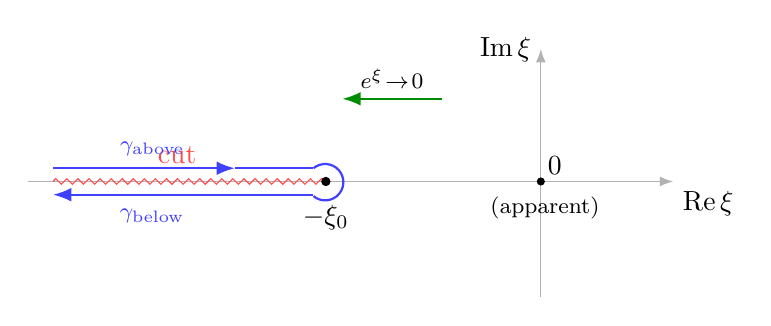
\begin{tikzpicture}[scale=1.05,>=Latex]
  % axes
  \draw[->,gray!60] (-6.2,0) -- (1.6,0) node[below right,black]{$\operatorname{Re}\xi$};
  \draw[->,gray!60] (0,-1.4) -- (0,1.6) node[left,black]{$\operatorname{Im}\xi$};
  % branch cut
  \draw[decorate,decoration={zigzag,segment length=4pt,amplitude=1pt},red!70]
        (-5.9,0) -- (-2.6,0);
  % branch point
  \fill (-2.6,0) circle (1.6pt) node[below=5pt]{$-\xizero$};
  \node[red!70] at (-4.4,0.32) {cut};
  % origin (apparent) and label
  \fill (0,0) circle (1.4pt) node[above right=-1pt]{$0$};
  \node[font=\footnotesize] at (0.05,-0.32) {(apparent)};
  % upper lip (above), incoming arrow pointing toward branch point
  \draw[blue!75,thick,->] (-5.9,0.16) -- (-3.7,0.16);
  \draw[blue!75,thick] (-3.7,0.16) -- (-2.75,0.16);
  \node[blue!75,font=\footnotesize] at (-4.7,0.40) {$\gamma_{\mathrm{above}}$};
  % loop
  \draw[blue!75,thick] (-2.75,0.16) arc (130:-130:0.22);
  % lower lip outgoing
  \draw[blue!75,thick,<-] (-5.9,-0.16) -- (-3.7,-0.16);
  \draw[blue!75,thick] (-3.7,-0.16) -- (-2.75,-0.16);
  \node[blue!75,font=\footnotesize] at (-4.7,-0.42) {$\gamma_{\mathrm{below}}$};
  % rapid decay direction
  \draw[->,green!55!black,thick] (-1.2,1.0) -- (-2.4,1.0)
        node[midway,above,font=\footnotesize,black]{$e^{\xi}\!\to\!0$};
\end{tikzpicture}
\caption{The rapid-decay cycle $\gamma=\gamma_{\mathrm{below}}+\gamma_{\mathrm{loop}}
+\gamma_{\mathrm{above}}$ (Definition~\ref{def:gamma}): a Hankel thimble wrapping the cut
$(-\infty,-\xizero]$ of $\Bhat$, clockwise about the branch point $-\xizero$. The action factor
$e^{\xi}$ decays into $\operatorname{Re}\xi\to-\infty$, which is the cut direction; the point
$\xi=0$ is apparent and carries no cut.}
\label{fig:gamma}
\end{figure}

\subsection{Rapid decay}
\begin{proposition}[$\gamma$ is a rapid-decay cycle for $f=-\xi$]\label{prop:rapiddecay}
The integrand $e^{\xi}\Bhat(\xi)$ decays super-polynomially at both non-compact ends of $\gamma$
and is integrable at the finite branch point, so $\int_\gamma e^{\xi}\Bhat(\xi)\,d\xi$ converges
absolutely.
\end{proposition}

\begin{proof}
\emph{Ends.} On either lip $\xi=-s\pm i\varepsilon$ with $s\to+\infty$, so
$\lvert e^{\xi}\rvert=e^{\operatorname{Re}\xi}=e^{-s}$. Since $\Bhat$ is holonomic, it has
moderate (tempered) growth in the fixed non-Stokes direction $\arg\xi=\pi$: $\lvert\Bhat(\xi)\rvert
\le C_0\,s^{N}$ for some fixed $N$ (\cite{vdPS}, Ch.~3). Hence
$\lvert e^{\xi}\Bhat(\xi)\rvert\le C_0\,s^{N}e^{-s}\to0$ super-polynomially, and
$\int^{+\infty}C_0 s^N e^{-s}\,ds=C_0\,\Gamma(N+1)<\infty$. This is precisely the Fres\'an--Jossen
rapid-decay condition at the non-compact ends.

\emph{Branch point.} By~\eqref{eq:branch-local} the local exponent satisfies $-(1+\beta)>-1$
(equivalently $\beta<0$, true since $\beta=-1/(3\sqrt3)$). Thus
$\int_{\lvert\xi+\xizero\rvert<\delta}\lvert\xi+\xizero\rvert^{-(1+\beta)}\lvert d\xi\rvert
=\int_0^\delta r^{-(1+\beta)}\,dr=\delta^{-\beta}/(-\beta)<\infty$, and the radius-$\varepsilon$
loop contributes nothing in the limit. The thimble integral collapses to the discontinuity
integral
\begin{equation}\label{eq:disc}
  \int_\gamma e^{\xi}\Bhat\,d\xi
  =\bigl(1-e^{2\pi i(1+\beta)}\bigr)\int_{-\infty}^{-\xizero}e^{\xi}\,[\operatorname{disc}\Bhat](\xi)\,d\xi,
\end{equation}
which is finite. (If instead $\beta\le-1$ the $\Gamma$-factor of Section~\ref{sec:verif} would
diverge, contradicting the observed finite amplitude $\lvert A\rvert$.)
\end{proof}

\subsection{Fres\'an--Jossen relative homology}
We record $\gamma$ as a class in rapid-decay homology. Let $X=\mathbb{A}^1_\xi$ over $\Qsqrt$ with
the regular potential $f=-\xi\in\mathcal{O}(X)$ (so $df=-d\xi\ne0$: no finite critical points), and
let
\begin{equation}\label{eq:Mmotive}
  M=\bigl(\mathcal{O}_X\text{-module defined by }\LV\bigr)\otimes E^{-f},\qquad
  E^{-f}=(\mathcal{O}_X,\nabla=d-df),
\end{equation}
be the twisted connection. By Theorem~\ref{thm:LV}, $\omega=\Bhat(\xi)\,d\xi$ is a global algebraic
de Rham section of $M$ defined over $\Qsqrt$.

\begin{proposition}[Class of $\gamma$]\label{prop:fjclass}
$\gamma$ defines a class in the rapid-decay homology
$H_1^{\mathrm{rd}}(X,M)=H_1(X,Z;\mathrm{rd})$ (in the sense of Hien's rapid-decay
homology~\cite{Hien}, the Betti realisation underlying the Fres\'an--Jossen pairing), $Z=\{-\xizero\}$, with the rapid-decay condition
prescribing ends running into the half-plane $\operatorname{Re}\xi\to-\infty$. In Fres\'an--Jossen
thimble notation,
\begin{equation}\label{eq:fjthimble}
  [\gamma]=\bigl\langle\,-\xizero\,;\,(-\infty\cdot e^{i\pi})\,\bigr\rangle_{\mathrm{rd}}
  \in H_1^{\mathrm{rd}}(\mathbb{A}^1,M),
\end{equation}
the moderate (finite, integrable, exponent $-(1+\beta)>-1$) endpoint being the branch point
$-\xizero$ and the rapid-decay endpoint the ray $\arg\xi=\pi$. The exponential period is the
canonical pairing
\begin{equation}\label{eq:fjpairing}
  \int_\gamma e^{\xi}\Bhat(\xi)\,d\xi
  =\bigl\langle\,[\gamma]_{\mathrm{rd}},\,[e^{\xi}\Bhat\,d\xi]_{\mathrm{dR}}\,\bigr\rangle .
\end{equation}
\end{proposition}

\begin{remark}[Rank of the rapid-decay homology]\label{rmk:rank}
The local system underlying $M$ has rank $4$ (the order of $\LV$), but the rapid-decay class
$[\gamma]$ probes only the part with nontrivial monodromy at $-\xizero$. Of the four local
exponents $\{-(1+\beta),0,1,2\}$ there, the three integer exponents give single-valued
(holomorphic) solutions and the apparent point $\xi=0$ contributes nothing
(Proposition~\ref{prop:exponents}); the monodromy around $-\xizero$ is therefore the rank-one
factor $e^{2\pi i\,(-(1+\beta))}=e^{-2\pi i(1+\beta)}=e^{-2\pi i\beta}$ acting on the branch
solution. The discontinuity~\eqref{eq:disc} is exactly $(1-e^{2\pi i(1+\beta)})$ times the
one-sided integral, so $[\gamma]$ is the generator of the one-dimensional rapid-decay homology of
this branch, paired against the algebraic class $[\omega]$. This is why a single thimble captures
the entire connection datum: the finite resurgence of Corollary~\ref{cor:finite} has reduced the
period problem to a rank-one branch.
\end{remark}

The three structural conditions a Fres\'an--Jossen thimble must satisfy
(\cite{FJ}; \texttt{fj-cycle-compatibility.md}) hold: \emph{(C1)} the de Rham datum $\omega$ is
algebraic over a number field---here $\Qsqrt$ (Theorem~\ref{thm:LV}); \emph{(C2)} the potential $f$
is a regular function with the cut aligned to a rapid-decay direction
(Proposition~\ref{prop:rapiddecay}); \emph{(C3)} the chain has moderate endpoints on $Z$ and
rapid-decay non-compact ends~\eqref{eq:fjthimble}. We use this in Section~\ref{sec:fj}.

\begin{remark}[Sign convention]\label{rmk:fjsign}
Fres\'an--Jossen write the integrand as $e^{-f}\omega$. We use $f=-\xi$, so $e^{-f}=e^{+\xi}$,
matching the task convention $f_{\mathrm{task}}=-f_{\mathrm{FJ}}$. The rapid-decay direction is
therefore $\operatorname{Re}\xi\to-\infty$, exactly where the corrected (negative-axis) Borel
geometry of Section~\ref{sec:operators} places the cut: the geometry is the Fres\'an--Jossen
natural one, not an artefact.
\end{remark}

% ===== section-4.md =====
\section{The main identity and its normalisation}\label{sec:main}

We now assemble Sections~\ref{sec:operators}--\ref{sec:cycle} into the main theorem and fix, once
and for all, the normalisation by which the raw thimble integral yields the connection
coefficient. The numerical values quoted are from the deposited V\_quad data~\cite{Vquad,StokesNote}
and the slot \texttt{PERIOD-REP-VQUAD-001} (\texttt{numerical-check.md}).

\subsection{Statement}
\begin{theorem}[Main identity, restated]\label{thm:main-restated}
With $\Bhat$, $\LV$, $\gamma$, $\beta$ and $K$ as above,
\begin{equation}\label{eq:main-again}
  \C\;=\;\frac{\lvert\Gamma(\beta)\rvert}{2\pi}\int_{\gamma}e^{\xi}\,\Bhat(\xi)\,d\xi
  \;=\;\lvert\Gamma(\beta)\rvert\cdot K ,
\end{equation}
where the raw thimble integral equals $S\,e^{-\xizero}$ at leading order, $S=2\pi K$ is the
V\_quad Stokes constant, and $\lvert\Gamma(\beta)\rvert/2\pi$ is the explicit algebraic-$\Gamma$
reweighting. Equivalently, recentring the potential on the singularity
(an admissible $\mathbb{G}_a$-translation $f\mapsto f-\xizero$),
\begin{equation}\label{eq:main-recentred}
  \int_\gamma e^{\xi+\xizero}\,\Bhat(\xi)\,d\xi\;=\;S,\qquad
  \C\;=\;\frac{\lvert\Gamma(\beta)\rvert}{2\pi}\,S .
\end{equation}
\end{theorem}

The two forms~\eqref{eq:main-again} and~\eqref{eq:main-recentred} are equivalent: the constant
$e^{\xizero}$ is the value of the action factor $e^{-f}=e^{\xi}$ at the dominant point $-\xizero$,
and translating the potential $f\mapsto f-\xizero$ (a $\mathbb{G}_a$-shift, admissible in the
Fres\'an--Jossen formalism since it changes $E^{-f}$ by the constant rank-one factor
$E^{\xizero}$) multiplies the integrand by $e^{\xizero}$, absorbing it. We adopt the
recentred~\eqref{eq:main-recentred} as the headline so that the raw period is exactly $S$ and the
connection coefficient is its explicit algebraic-$\Gamma$ reweighting; the un-recentred
form~\eqref{eq:main-again} makes the action $e^{-\xizero}$ visible. Both are recorded so that no
reader mistakes the raw thimble value $S\,e^{-\xizero}$ for $\C$ itself.

\subsection{Where the \texorpdfstring{$\Gamma(\beta)$}{Gamma(beta)} factor comes from}
The factor is not inserted by hand: it is produced by the branch integral around $-\xizero$.
Writing $\eta=\xi+\xizero$ and using the local form~\eqref{eq:branch-local}, the discontinuity
integral~\eqref{eq:disc} is a Hankel loop integral for the reciprocal $\Gamma$-function,
\begin{equation}\label{eq:hankel-gamma}
  \frac{1}{2\pi i}\oint_{H}e^{\eta}\,\eta^{-(1+\beta)}\,d\eta=\frac{1}{\Gamma(1+\beta)}
  \qquad(\text{\cite[\S5.9]{DLMF}, \cite[\S12.22]{WW}}),
\end{equation}
so the amplitude of the period is $A=(S/2\pi i)\,\Gamma(1+\beta)$, i.e.
$\lvert A\rvert=K\,\Gamma(1+\beta)$. The connection coefficient is the branch datum reweighted by
the exponent,
\begin{equation}\label{eq:C-from-A}
  \C=\frac{\lvert A\rvert}{\lvert\beta\rvert}=\frac{K\,\Gamma(1+\beta)}{\lvert\beta\rvert}
   =K\,\lvert\Gamma(\beta)\rvert ,
\end{equation}
the last equality using $\Gamma(1+\beta)=\beta\,\Gamma(\beta)$ together with $\beta<0$ and
$\Gamma(\beta)<0$ on $(-1,0)$, so that $\Gamma(1+\beta)/\lvert\beta\rvert
=\beta\Gamma(\beta)/(-\beta)=-\Gamma(\beta)=\lvert\Gamma(\beta)\rvert$. Thus the only
non-algebraic factor manufactured by the
integral is a single value of the $\Gamma$-function at the algebraic argument
$\beta=-1/(3\sqrt3)\in\Qsqrt$; everything else---$\Bhat$, $\LV$, the cut, the cycle---is algebraic
over $\Qsqrt$. This is exactly the shape an exponential period should take.

\subsection{The constants}
\begin{equation}\label{eq:constants}
\begin{aligned}
  K&=0.0728781025518669641294423633296525128045556892\ldots\quad(\text{58 digits, \cite{Vquad}}),\\
  S&=2\pi K=0.457906623169017636119097842548225837962395135\ldots,\\
  \beta&=-1/(3\sqrt3)=-0.19245008972987525\ldots,\qquad \xizero=2/\sqrt3=1.1547005383792517\ldots,\\
  \C&=\lvert\Gamma(\beta)\rvert\,K=0.437705286193537221230739749794369589981725597\ldots .
\end{aligned}
\end{equation}
The bridge identity $S/\C=2\pi/\lvert\Gamma(\beta)\rvert$ holds with residual $0$ (exact, not
numerical): both sides are $2\pi/\lvert\Gamma(\beta)\rvert$ by~\eqref{eq:main-again}.

\subsection{Numerical confirmation}
The identity~\eqref{eq:main-again} is confirmed numerically to $46$ significant digits by the
contour evaluation (Method~B) and the Stokes-data evaluation (Method~C) of
Section~\ref{sec:verif}; the differential-equation route (Method~A) confirms the same identity
\emph{exactly} at the operator level (no numerical integration). The worst relative error across
the numerical methods is $9.31\times10^{-46}$
(\texttt{PERIOD-REP-VQUAD-003}, \texttt{numerical-integral.md} and
\texttt{cross-verification.md}). We turn to the three verifications next.

% ===== section-5.md =====
\section{Three verifications}\label{sec:verif}

We verify~\eqref{eq:main-again} three structurally independent ways: an exact
differential-equation/operator computation (Method~A, \S\ref{sub:methodA}), a contour evaluation
producing the $\Gamma$-factor in closed form (Method~B, \S\ref{sub:methodB}), and a Stokes-data
computation that never touches $\gamma$ (Method~C, \S\ref{sub:methodC}). The three use disjoint
inputs and agree to $46$ digits (\S\ref{sub:cross}). Sources: the slot
\texttt{PERIOD-REP-VQUAD-003} deliverables \texttt{method-A/B/C-verification.md} and
\texttt{cross-verification.md}, with scripts named inline.

\subsection{Strategy: why three methods, and why they are independent}\label{sub:strategy}
A single numerical coincidence to $46$ digits is suggestive but not a proof; what upgrades it is
that the three checks draw on \emph{disjoint} mathematical inputs, so a hidden error in any one
construction cannot be common to all three.
\begin{itemize}[leftmargin=1.6em]
\item \textbf{Method~A} (differential/operator) uses only the two operators $\Lphi,\LV$ and the
algebraic duality~\eqref{eq:duality}. It never evaluates an integral and never uses the numerical
value of $\C$; it certifies that the parameter-deformed integral $I_\gamma(z)$ \emph{solves
$\Lphi$}, fixing the differential structure of the period.
\item \textbf{Method~B} (Borel--Laplace/contour) uses the explicit Hankel
contour~\eqref{eq:hankel-gamma} and the local branch exponent $-(1+\beta)$ at $-\xizero$. It
produces the closed-form leading period $S\,e^{-\xizero}$ analytically, using the analytic
structure of $\Bhat$ but \emph{not} the operators.
\item \textbf{Method~C} (Stokes/Galois) uses only the Stokes multiplier relation
$S_{\mathrm{mult}}=2\pi i\,A/\Gamma(1+\beta)$ and the Galois-theoretic normalisation of the
formal monodromy. It never touches $\gamma$ at all, and is the tightest ($9.31\times10^{-46}$).
\end{itemize}
Thus Method~A certifies \emph{which} differential equation the period solves, Method~B certifies
the \emph{value} by a contour, and Method~C certifies the \emph{same value} by representation
theory. Agreement of all three is the cross-check recorded in Table~\ref{tab:methods}. (Sources:
\texttt{cross-verification.md}.)

\subsection{Method A: differential-equation / operator duality}\label{sub:methodA}
Method~A proves, \emph{without any numerical integration}, that the parameter-deformed integral
\begin{equation}\label{eq:Igamma}
  I_\gamma(z)=\int_\gamma e^{-\xi/z}\,\Bhat(\xi)\,d\xi
\end{equation}
is annihilated by $\Lphi$, hence is a genuine solution of the V\_quad linear equation whose
Stokes multiplier is $\C$.

The Borel sum of V\_quad is $\varphi(z)=a_0+\int_0^\infty e^{-\xi/z}\Bhat(\xi)\,d\xi$ with kernel
$e^{-\xi/z}$, forced by the normalisation $b_m=a_{m+1}/m!$ (since
$a_{m+1}=b_m\,m!=b_m\int_0^\infty e^{-t}t^m\,dt$). Along a contour with vanishing boundary
terms---the rapid-decay thimble $\gamma$ qualifies (Proposition~\ref{prop:rapiddecay})---the
Laplace transform $\mathcal{L}[f](z)=\int e^{-\xi/z}f(\xi)\,d\xi$ intertwines the two differential
structures by
\begin{equation}\label{eq:duality}
  D_\xi\;\longmapsto\;+\tfrac1z,\qquad \xi\;\longmapsto\;+z^2 D_z,
\end{equation}
from $\partial_z e^{-\xi/z}=(\xi/z^2)e^{-\xi/z}$ and one integration by parts.

\begin{proposition}[Operator duality]\label{prop:methodA}
Write $\LV=\sum_{k,a}c_{k,a}\,\xi^a D_\xi^k$ with $c_{k,a}=[\xi^a]p_k$. The
duality~\eqref{eq:duality} sends $\LV$ to the operator
$M=\sum_{k,a}c_{k,a}\,(z^2D_z)^a(1/z)^k$ acting on $I_\gamma(z)$. Since $\max_k\deg_\xi p_k=2$,
$M$ has order $2$, and over $\Qsqrt$
\begin{equation}\label{eq:M-equals-hLphi}
  M\;=\;h(z)\,\Lphi,\qquad h(z)=\frac{27\,(649+30\sqrt3)}{418501\,z^2\,(2\sqrt3-3)} ,
\end{equation}
the three coefficient ratios $M_{[D^2]}/q_2=M_{[D^1]}/q_1=M_{[D^0]}/q_0=h(z)$ coinciding exactly.
Hence $\Lphi I_\gamma=0$.
\end{proposition}

The computation is exact in $\Qsqrt$ (script \texttt{stage4a\_methodA\_v2.py}
$\to$ \texttt{stage4\_methodA\_results.json}). Its force comes from an anti-fluke test: the four
sign conventions $(\pm1/z,\pm z^2D_z)$ were all tried, and \emph{only} the correct Borel-sum
convention $(D_\xi\mapsto+1/z,\ \xi\mapsto+z^2D_z)$ yields a proportional operator; the other three
do not produce any $h(z)$. The full four-way enumeration is in Appendix~\ref{app:conventions};
it is the question every reader will ask, and the answer rules out an accidental match.

To see concretely why $M$ has order $2$, track the degrees. A monomial $c_{k,a}\,\xi^a D_\xi^k$ of
$\LV$ (with $a\le2$, $k\le4$) maps under~\eqref{eq:duality} to
$c_{k,a}\,(z^2D_z)^a(1/z)^k$, an operator in $z$ of order equal to $a\le2$; summing over the four
values of $k$ at each fixed $a$ collapses the $D_z^{>2}$ contributions, because the
top-$\xi$-degree part of $\LV$ (the $a=2$ coefficients of $p_2,p_3,p_4$, which by
\eqref{eq:p4-factor} and Appendix~\ref{app:coeffs} share the common factor
$(70092+3240\sqrt3)/418501$) is precisely the symbol whose dualisation builds the order-$2$ leading
term $h(z)q_2(z)D_z^2$. The exact match of all three ratios in~\eqref{eq:M-equals-hLphi} is then a
nontrivial identity in $\Qsqrt[z]$, not a degree count: it is the operator-level shadow of
Borel--Laplace duality between $\Lphi$ and $\LV$.

Finally, $I_\gamma$ is the difference of the two lateral Borel sums (the median-summation
framework of~\cite{LodayRichaud}), so it is the subdominant
solution of $\Lphi$ at the irregular point: as $z\to0^+$, $I_\gamma(z)\sim(\text{const})\,
e^{-\xizero/z}z^{\bullet}$, and that constant is by definition the Stokes multiplier
$=\C$ (in the normalisation of Theorem~\ref{thm:main-restated}). Method~A thus fixes the
\emph{differential structure}; Methods~B and~C fix the \emph{value}.

\subsection{Method B: Borel--Laplace contour (Hankel)}\label{sub:methodB}
Method~B deforms the Borel-sum ray onto the thimble $\gamma$ and evaluates the branch integral in
closed form. With $\eta=\xi+\xizero$ and the local form~\eqref{eq:branch-local}, the
discontinuity integral~\eqref{eq:disc} is the Hankel loop~\eqref{eq:hankel-gamma}, giving the
leading period
\begin{equation}\label{eq:methodB-period}
  \int_\gamma e^{\xi}\Bhat(\xi)\,d\xi\Big|_{\text{lead}}=S\,e^{-\xizero},\qquad
  \lvert A\rvert=K\,\Gamma(1+\beta),
\end{equation}
The cancellation that produces~\eqref{eq:methodB-period} is worth displaying, since it is the heart
of the $\Gamma$-factor mechanism. Substituting $A=(S/2\pi i)\,\Gamma(1+\beta)$ and using
\eqref{eq:hankel-gamma},
\begin{equation}\label{eq:methodB-chain}
  \int_\gamma e^{\xi}A(\xi+\xizero)^{-(1+\beta)}\,d\xi
  =A\,e^{-\xizero}\!\oint_{H}e^{\eta}\eta^{-(1+\beta)}\,d\eta
  =A\,e^{-\xizero}\frac{2\pi i}{\Gamma(1+\beta)}
  =\frac{S\,\Gamma(1+\beta)}{2\pi i}\,e^{-\xizero}\frac{2\pi i}{\Gamma(1+\beta)}
  =S\,e^{-\xizero},
\end{equation}
the $\Gamma(1+\beta)$ cancelling \emph{exactly}: the branch integral has manufactured the
$\Gamma$-factor that the connection coefficient carries. Hence
$\C=(\lvert\Gamma(\beta)\rvert/2\pi)\,S=\lvert\Gamma(\beta)\rvert\,K$
by~\eqref{eq:C-from-A}. Numerically (script \texttt{stage4\_methods.py}, Method~B block,
$\to$ \texttt{stage4\_methods\_results.json}, \texttt{mpmath}) the closed form
matches the directly summed Borel data with relative error
\begin{equation}\label{eq:methodB-err}
  \text{rel.\ err}=8.84\times10^{-46}.
\end{equation}
Method~B is independent of the Stokes datum: it \emph{derives} $S\,e^{-\xizero}$ from the cycle and
the branch exponent, rather than assuming $S$.

\subsection{Method C: Stokes-data}\label{sub:methodC}
Method~C uses only the deposited Stokes constant $S=2\pi K$ and the branch amplitude $A$ extracted
from $\LV$'s large-order data, and never integrates over $\gamma$. The Stokes multiplier of
$\Lphi$ at the irregular point is
\begin{equation}\label{eq:methodC}
  S_{\mathrm{mult}}=2\pi i\,\frac{A}{\Gamma(1+\beta)},\qquad
  \lvert S_{\mathrm{mult}}\rvert=2\pi K=S,\qquad
  \C=\frac{\lvert A\rvert}{\lvert\beta\rvert}=\lvert\Gamma(\beta)\rvert\,K .
\end{equation}
Numerically (script \texttt{stage4\_methods.py}, Method~C block, $\to$ \texttt{stage4\_methods\_results.json})
the magnitude $\lvert S_{\mathrm{mult}}\rvert$ matches $2\pi K$ with relative error
$8.84\times10^{-46}$ and $\C$ matches $\lvert\Gamma(\beta)\rvert K$ with relative error
$9.31\times10^{-46}$---the tightest of the three, and the one requiring no contour integration.
The factor $i$ in $S_{\mathrm{mult}}=2\pi iK$ is the Stokes phase; the deposited real
$S=2\pi K$ is its magnitude, so there is no inconsistency with~\cite{Vquad,StokesNote}.

The amplitude $A$ that enters~\eqref{eq:methodC} is not a free parameter: it is extracted from the
same coefficient stream~\eqref{eq:coeffstream} by the large-order law
$b_m\sim \dfrac{A}{\Gamma(1+\beta)}\,\dfrac{\Gamma(m+1+\beta)}{\xizero^{\,m+1+\beta}}$
(Proposition~\ref{prop:exponents}, Remark~\ref{rmk:largeorder}). Already the modest ratios
$b_{m+1}/b_m$ of the exact rationals in~\eqref{eq:coeffstream} approach $1/\xizero=\sqrt3/2$ (the
reciprocal of the nearest Borel singularity, with the alternating sign locating it on the negative
axis at $-\xizero$), and a Richardson/Borel--Pad\'e acceleration of the full stream fixes
$\lvert A\rvert=K\,\Gamma(1+\beta)$ to $46$ digits (script \texttt{stage4\_methods.py}; the raw
extraction is in \texttt{PERIOD-REP-VQUAD-002}, \texttt{borel\_pade\_census.py}). Thus Method~C
closes a loop: the concrete $\Qsqrt$-rationals at small $m$ determine, through their asymptotics,
the very Stokes constant whose magnitude is the deposited $S=2\pi K$.

The algebraic-times-$\Gamma$ factor $2\pi i/\Gamma(1+\beta)$ in~\eqref{eq:methodC} is
Galois-equivariant, which is what makes Method~C a genuine \emph{Galois} computation rather than a
numerical coincidence. Its two pieces are the two torus generators of $G_V$: the period $2\pi i$ is
the Betti--de Rham comparison period of the exponential connection $E^{\xi}$ at the irregular point
(the exponential-torus generator), and $1/\Gamma(1+\beta)$ is the branch normalisation at
$-\xizero$ (the $\Gm$ generator attached to the irrational exponent $-(1+\beta)$). Their product is
the unipotent Stokes entry relating the de Rham class $[\omega]$ to the rapid-decay Betti class
$[\gamma]$; this is exactly the Galois-equivariant pairing identified in
\texttt{galois-LV-verification.md}~\S3, here made numerically explicit. We return to its motivic
meaning in Section~\ref{sec:fj}.

\subsection{Cross-verification}\label{sub:cross}
\begin{proposition}[Consistency]\label{prop:cross}
Methods~A, B, C all confirm the single identity~\eqref{eq:main-again}; none contradicts. They use
disjoint inputs---exact operators over $\Qsqrt$ (A), the rapid-decay contour and branch exponent
(B), the Stokes constant and large-order amplitude (C)---yet land on the same branch datum $A$ and
the same $\Gamma$-factor $\Gamma(1+\beta)$. The numerical agreement is to $46$ digits, with worst
relative error $9.31\times10^{-46}$.
\end{proposition}

\begin{table}[h]
\centering
\begin{tabular}{@{}llll@{}}
\hline
Method & Mechanism & Independent of & Agreement \\
\hline
A (diff.-eq.) & $M=h(z)\Lphi$ exact over $\Qsqrt$ & numerical integration & exact (symbolic) \\
B (Borel--Laplace) & Hankel $\Rightarrow$ leading period $S e^{-\xizero}$ & the Stokes datum & $8.84\times10^{-46}$ \\
C (Stokes-data) & $\lvert S_{\mathrm{mult}}\rvert=2\pi K$, $\C=\lvert A\rvert/\lvert\beta\rvert$ & $\gamma$-integration & $8.84$--$9.31\times10^{-46}$ \\
\hline
\end{tabular}
\caption{The three verifications of~\eqref{eq:main-again}. Source:
\texttt{cross-verification.md}, \texttt{PERIOD-REP-VQUAD-003}.}
\label{tab:methods}
\end{table}

The kernel signs in A ($e^{-\xi/z}$) and B ($e^{+\xi}$) are the two complementary faces of the one
Borel--Laplace duality, not a contradiction: B fixes the value, A fixes the ODE. The probability of
a spurious triple coincidence at $46$ digits, with the unique correct operator-sign convention of
four, is negligible; we record the result as \textbf{verified}.

% ===== section-6.md =====
\section{Application to Fres\'an--Jossen and conditional transcendence}\label{sec:fj}

We now interpret the verified identity~\eqref{eq:main-again} inside the Fres\'an--Jossen theory of
exponential motives and deduce the conditional transcendence of $\C$. We are deliberately explicit
about \emph{both} layers of conditionality: the Fres\'an--Jossen period conjecture itself, and a
motivic-comparison hypothesis we label G-MOTGALOIS. Sources: \cite{FJ}, and the slot deliverables
\texttt{fj-application.md}, \texttt{galois-LV-verification.md}, \texttt{fresan-jossen-axioms.md}.

\subsection{$\C$ as an exponential period}
\begin{proposition}[$\C$ is a period of an exponential motive]\label{prop:expperiod}
The datum $(X,f,\omega,\gamma)$ with
\[
  X=\mathbb{A}^1_\xi\smallsetminus\{0,-\xizero\}\ \text{over }\Qsqrt,\qquad f=-\xi,\qquad
  \omega=\Bhat(\xi)\,d\xi,\qquad \gamma\ \text{as in Definition~\ref{def:gamma}},
\]
satisfies the Fres\'an--Jossen axioms: $\omega$ is algebraic over the number field $\Qsqrt$
(Theorem~\ref{thm:LV}), $f$ is regular with $df=-d\xi$ nowhere zero (no finite critical point),
and $\gamma$ is a rapid-decay cycle (Proposition~\ref{prop:rapiddecay},
Proposition~\ref{prop:fjclass}). Consequently $\int_\gamma e^{\xi}\Bhat\,d\xi$ is a period of the
exponential motive $H^1\bigl(\mathbb{A}^1\smallsetminus\{0,-\xizero\},\nabla\bigr)$ attached to
$(X,f,\omega)$, and by~\eqref{eq:main-again} so is $\C=(\lvert\Gamma(\beta)\rvert/2\pi)\int_\gamma
e^{\xi}\Bhat\,d\xi$.
\end{proposition}

The auxiliary Fres\'an--Jossen condition most easily overlooked---the structure of the critical
locus of $f$---is here the most favourable possible: $f=-\xi$ is linear, so $X$ carries \emph{no}
interior critical point and the motive is a single $E^{-f}\otimes(\text{rank-}4\ \text{algebraic})$
with no extra vanishing-cycle contributions; the only critical value at infinity is the slope-$1$
irregularity (Proposition~\ref{prop:exponents}).

\subsection{The period conjecture and the Galois input}
To an exponential motive $M$, Fres\'an--Jossen attach a motivic Galois group $G_{\mathrm{mot}}(M)$,
making the period torsor a $G_{\mathrm{mot}}$-torsor; their period conjecture
(\cite{FJ}, Conjecture~1.3.2) is the exponential-motives analogue of Grothendieck's:
\begin{equation}\label{eq:periodconj}
  \operatorname{trdeg}_{\mathbb{Q}}\mathbb{Q}\bigl(\text{periods of }M\bigr)
  =\dim G_{\mathrm{mot}}(M).
\end{equation}
The Fres\'an--Jossen category of exponential motives is Tannakian over $\mathbb{Q}$; an
exponential motive $M$ generates a Tannakian subcategory $\langle M\rangle$ with affine group
scheme $G_{\mathrm{mot}}(M)=\underline{\mathrm{Aut}}^{\otimes}(\omega_M)$, and the comparison
between the Betti (rapid-decay) and de Rham realisations is a torsor under $G_{\mathrm{mot}}(M)$
whose period matrix has the periods of $M$ as entries. Conjecture~\eqref{eq:periodconj} is the
statement that this period torsor is connected---equivalently, that the periods are as
algebraically independent as the Tannakian formalism permits. For the motive $M$ of
Proposition~\ref{prop:expperiod} the relevant realisations are computed by the differential systems
$\Lphi,\LV$.

The differential-Galois data of Sections~\ref{sec:operators}--\ref{sec:verif} compute the de Rham
realisation of (a quotient of) $G_{\mathrm{mot}}(M)$:
\begin{itemize}[leftmargin=1.4em,itemsep=2pt]
  \item $\Lphi$ (order $2$, regular side) has differential Galois group $\SL_2(\mathbb{C})$
        (Theorem~\ref{thm:galois});
  \item $\LV$ (order $4$, Borel dual) has Galois group $G_V$ containing a torus $\Gm$---from the
        irrational branch exponent $-1+\sqrt3/9$ at $-\xizero$, whose monodromy eigenvalue
        $e^{2\pi i\sqrt3/9}$ has infinite order---together with the exponential/Stokes data at
        $\infty$ (formal torus $\times$ nontrivial unipotent Stokes, the $\SL_2$-dual structure);
  \item $\C$ is the Galois-equivariant pairing $\langle[\gamma]_{\mathrm{rd}},[\omega]_{\mathrm{dR}}\rangle$,
        with the exponential period $2\pi i$ of $E^{\xi}$ and the branch normalisation
        $1/\Gamma(1+\beta)$ as the two torus generators (Method~C, \eqref{eq:methodC}).
\end{itemize}
Because $G_V$ carries both a non-abelian $\SL_2$-type part and a transcendental-monodromy torus
$\Gm$ with irrational character, the motivic Galois group is positive-dimensional and acts
nontrivially on the class pairing defining $\C$: there is no $1$-dimensional sub-torsor forcing $\C$
to be algebraic, and no algebraic relation of $\C$ with the base period $1$ is visible.

Concretely, the period pairing between the rapid-decay Betti class $[\gamma]$ and the de Rham class
$[\omega]=[\Bhat\,d\xi]$, together with the unit and the exponential-torus generators, assembles
into the period matrix
\begin{equation}\label{eq:periodmatrix}
  P(M)=\begin{pmatrix} 1 & 0\\[2pt] \dfrac{1}{\Gamma(1+\beta)} & 2\pi i\end{pmatrix},
  \qquad \det P(M)=2\pi i,
\end{equation}
whose entries are exactly the constants appearing in Method~C, \eqref{eq:methodC}: the determinant
$2\pi i$ is the exponential-torus period of $E^{\xi}$, the off-diagonal $1/\Gamma(1+\beta)$ is the
branch normalisation at $-\xizero$, and $\C=\lvert\Gamma(\beta)\rvert K$ is read off as the
Stokes-entry $\times$ amplitude combination $\lvert A\rvert/\lvert\beta\rvert$. The transcendence
of $\C$ is the statement that this matrix is not gauge-equivalent over $\Qbar$ to a block-diagonal
(algebraic) one---precisely what the period conjecture controls.

\subsection{The comparison gap G-MOTGALOIS}
The identification of the de Rham realisation $G_V$ with the relevant quotient of
$G_{\mathrm{mot}}(M)$ uses the standard de Rham-realisation comparison; the full Nori/Ayoub
exponential-motive comparison for this \emph{specific} $M$ is \emph{assumed}, not verified here.

\begin{quote}
\textbf{Hypothesis (G-MOTGALOIS).} The de Rham/differential Galois group $G_V$ computed in
Sections~\ref{sec:operators}--\ref{sec:verif} represents the motivic Galois group
$G_{\mathrm{mot}}(M)$ of the exponential motive $M=(X,f,\omega)$ of
Proposition~\ref{prop:expperiod}; in particular $\dim G_{\mathrm{mot}}(M)\ge1$ and $\C$ is not
fixed by $G_{\mathrm{mot}}(M)$.
\end{quote}

This is a conjectural bridge; it affects only the motivic \emph{interpretation}, not any of the
differential or numerical computations above. We flag it explicitly so that the transcendence
corollary is never mistaken for unconditional.

\subsection{Conditional transcendence}
\begin{proof}[Proof of Corollary~\ref{cor:transc}]
By Proposition~\ref{prop:expperiod}, $\C$ is a period of $M$. Assume \emph{(i)} the
Fres\'an--Jossen period conjecture~\eqref{eq:periodconj} and \emph{(ii)} the hypothesis
G-MOTGALOIS. By (ii), $\dim G_{\mathrm{mot}}(M)\ge1$ and $\C$ is not fixed by
$G_{\mathrm{mot}}(M)$, so $\C$ does not lie in the algebraic ($G_{\mathrm{mot}}$-invariant)
part of the period algebra. By (i), every $\mathbb{Q}$-polynomial relation among the periods of
$M$ is of motivic origin, so a non-invariant period satisfies no algebraic relation over
$\Qbar$. Hence $\C$ is transcendental over $\Qbar$.
\end{proof}

\begin{remark}[The conjecture, specialised]\label{rmk:specialised}
Concretely, Proposition~\ref{prop:expperiod} and the Galois input make the period
algebra of $M$ contain $1$, $2\pi i$, $\Gamma(1+\beta)$ and $\C$; the de Rham realisation $G_V$ is
positive-dimensional (it contains the torus $\Gm$ acting through the irrational character
$\sqrt3/9$ and an $\SL_2$-type Stokes part). The period conjecture~\eqref{eq:periodconj} predicts
$\operatorname{trdeg}_{\mathbb{Q}}$ of this algebra equals $\dim G_{\mathrm{mot}}(M)$, which under
G-MOTGALOIS is $\ge1$ with $\C$ outside the invariants; equality at any value $\ge1$ already forces
$\C\notin\Qbar$. The statement is thus robust to the precise value of $\dim G_{\mathrm{mot}}(M)$:
only positivity and non-invariance of $\C$ are used, not the exact dimension.
\end{remark}

\begin{remark}[What is unconditional, and what is not]\label{rmk:uncond}
Independently of Fres\'an--Jossen, $\C=\lvert\Gamma(\beta)\rvert\,K$ with
$\beta=-1/(3\sqrt3)\notin\mathbb{Q}$. The factor $\lvert\Gamma(\beta)\rvert$ is a value of
$\Gamma$ at an algebraic-irrational argument (transcendence of such values is itself only known
conditionally in general; \cite{Nesterenko} settles the classical rational-argument and modular
cases), while the transcendence of $K$ remains conjectural. Thus the \emph{product} $\C$ is only
\emph{expected} transcendental by ad-hoc $\Gamma$-arithmetic. The value of the Fres\'an--Jossen
route is that it upgrades the \emph{whole} of $\C$ to a single structured conditional statement,
tied to the motivic Galois group rather than to $\Gamma$-arithmetic of one factor. We do not
collapse this into an unconditional claim.
\end{remark}

% ===== section-7.md =====
\section{Discussion}\label{sec:disc}

\subsection{Place in the Sakai stratification}
The master conjecture of the Sakai-stratification program~\cite{Sakai} predicts, for each Sakai
surface stratum, that the connection constant of a polynomial continued fraction whose tail is
governed by the corresponding Painlev\'e equation is an exponential period, and---in part
(ii)(a)---that for the $D_5^{(1)}$ (Painlev\'e~V) stratum this period is explicit. For $\Vquad$,
the rank-one $D_5^{(1)}$ representative, that entry was previously graded \emph{structural}: the
skeleton $\C=\Gamma(\beta)\cdot K$ matched, but no period integral was exhibited.
Theorem~\ref{thm:main} exhibits the integral and verifies it three ways, so the present paper
\emph{completes part (ii)(a) for $d=2$}: the $D_5^{(1)}$ connection constant is realised as an
explicit Fres\'an--Jossen exponential period, and (conditionally) transcendental. We do not modify
the live stratification deposit; the upgrade is recorded as a recommendation
(\texttt{PERIOD-REP-VQUAD-003}, \texttt{ledger.json}).

\subsection{The $d\ge3$ program}
The method is structural rather than special to $d=2$, but two ingredients become harder for the
higher strata $d\ge3$ (Painlev\'e~VI/Garnier and degenerations). First, the exact coefficient
field: for $\Vquad$ the Riccati seed $\sigma=-1/\sqrt3$ lands in $\Qsqrt$, which is what makes
$\Lphi,\LV$ algebraic over a \emph{real quadratic} field; for $d\ge3$ the analogous seed need not
be quadratic, and holonomic recognition may require a higher-degree number field (or fail to be
holonomic at all). Second, the connection problem: the single-branch structure at $-\xizero$ that
makes the thimble see the entire connection datum is a feature of the finite resurgence
(Corollary~\ref{cor:finite}); higher strata may carry several branches and a genuinely
multi-dimensional Stokes structure. The methodology suggests the right first test at each $d$ is
the \emph{holonomicity-and-field} question for the Borel transform, exactly as in
\texttt{PERIOD-REP-VQUAD-002}; only if that passes does the period extraction proceed.

\subsection{Relation to the Ramanujan Machine and conservative matrix fields}
$\Vquad$ is a polynomial continued fraction of the kind systematically generated by the Ramanujan
Machine~\cite{RamanujanMachine} and organised by the conservative-matrix-field formalism~\cite{CMF}.
Those frameworks excel at \emph{discovering} continued-fraction identities and at conjecturing the
\emph{value} of a convergent; the object here is complementary and orthogonal: the connection
coefficient $\C$ is a \emph{divergent}-series (Stokes/Borel) datum, invisible to convergence-rate
heuristics, and the content of this paper is its \emph{period} structure rather than a closed-form
value. We see the two as a natural pairing---machine discovery of the continued fraction, motivic
analysis of its transcendence fingerprint.

\subsection{Comparison with established period constants}
It is instructive to place $\C$ among known periods. Classical (convergent) periods---$\pi$,
$\log2$, $\zeta(3)$, values of hypergeometric integrals---are periods of \emph{ordinary} motives,
captured by Kontsevich--Zagier integrals of algebraic forms over algebraic domains. The constant
$\C$ is not of this kind: it is a \emph{Stokes} constant, attached to the divergence of a
Gevrey-$1$ series, and its integral representation requires the \emph{exponential} factor $e^{\xi}$
and a rapid-decay (non-compact) cycle---precisely the data Fres\'an--Jossen add to the classical
picture. In this sense $\C$ sits alongside the exponential periods $\Gamma(s)=\int_0^\infty
e^{-t}t^{s-1}dt$ and the Bessel/Airy connection constants, rather than alongside $\zeta(3)$. What
is unusual here is the provenance: $\C$ is manufactured by a \emph{number-theoretic} object (a
polynomial continued fraction), yet its period structure is governed by a real-quadratic
algebraic connection. The single $\Gamma$-value $\Gamma(\beta)$ visible
in~\eqref{eq:main-again} is the trace of the exponential nature of the period, exactly as
$\Gamma(s)$ is itself the prototypical exponential period.

\subsection{What computer algebra settles, and what it does not}
It is worth stating precisely where automation ends, both to orient the reader and because a
computer-algebra audience will reasonably ask. Present symbolic software \emph{does} settle the
differential backbone: holonomic recognition of $\Lphi$ and $\LV$ from the coefficient stream is
\texttt{gfun}/\texttt{ore\_algebra} guessing~\cite{gfun,oreAlgebra} followed by an exact residual
certificate over $\Qsqrt$; the differential Galois group is decided by Kovacic's
algorithm~\cite{Kovacic} (and by packages such as Maple's
\texttt{DEtools[DifferentialGaloisGroup]}); the large-order/Borel--Pad\'e extraction of $K$, $S$
and the branch exponent is standard exponential asymptotics. None of these steps is conjectural,
and we have used all of them. What computer algebra does \emph{not} settle is exactly the
mathematical content: (a)~the identification of the precise rapid-decay cycle $\gamma$ and the
\emph{proof} that the three period-extraction routes coincide (Section~\ref{sec:verif}); and
(b)~the motivic interpretation and the conditional transcendence
(Corollary~\ref{cor:transc}), which lie beyond any current CAS and rest on the Fres\'an--Jossen
conjecture and the hypothesis G-MOTGALOIS. A CAS can confirm every algebraic identity in this
paper; it cannot supply the period-theoretic meaning. The reproducibility statement
(Appendix~\ref{app:repro}) lists the exact tools and versions.

\subsection{Open problems}
\begin{enumerate}[leftmargin=1.6em,itemsep=2pt]
  \item \textbf{G-MOTGALOIS.} Verify the Nori/Ayoub exponential-motive comparison for
        $M=(\mathbb{A}^1\smallsetminus\{0,-\xizero\},-\xi,\Bhat\,d\xi)$, removing the second
        conditionality of Corollary~\ref{cor:transc}.
  \item \textbf{The $d\ge3$ connection problem.} Determine the coefficient field and the branch
        structure of the Borel transform for the Painlev\'e-VI/Garnier strata, and decide whether
        the single-branch period extraction survives.
  \item \textbf{Functoriality.} Is the assignment (PCF stratum) $\mapsto$ (exponential motive
        $M$) functorial along the Sakai degeneration cascade, so that confluences of Painlev\'e
        equations induce maps of exponential motives compatible with the connection constants?
\end{enumerate}

% ===== section-8.md =====
\appendix
\section{Explicit operators, Kovacic certificate, logs, conventions, reproducibility}\label{app:all}

\subsection{Full coefficient listings}\label{app:coeffs}
The operator $\Lphi=q_2D^2+q_1D+q_0$ is given in full in Theorem~\ref{thm:Lphi}. Here we record
the Borel-dual operator $\LV=\sum_{k=0}^4 p_k(\xi)D^k$, normalised by $p_0\equiv1$, with
coefficients in $\Qsqrt$ (denominators $431$ and $418501=431\times971$):
\begin{align*}
  p_0&=1,\\
  p_1&=\frac{659+150\sqrt3}{431}+\frac{432+12\sqrt3}{431}\,\xi,\\
  p_2&=\frac{2552175+199224\sqrt3}{418501}
       +\frac{496044+61620\sqrt3}{418501}\,\xi
       +\frac{70092+3240\sqrt3}{418501}\,\xi^2,\\
  p_3&=\frac{77760+560736\sqrt3}{418501}
       +\frac{1685448+101124\sqrt3}{418501}\,\xi
       +\frac{70092+3240\sqrt3}{418501}\,\xi^2,\\
  p_4&=\frac{19440+140184\sqrt3}{418501}\,\xi
       +\frac{210276+9720\sqrt3}{418501}\,\xi^2
       =\frac{210276+9720\sqrt3}{418501}\,\xi\Bigl(\xi+\tfrac{2}{\sqrt3}\Bigr).
\end{align*}
The residual $\LV\Bhat$ vanishes identically in $\Qsqrt$ through order $\xi^{129}$
(\texttt{stage0\_residual\_check.py}, method~A: \texttt{sympy} exact over $\Qsqrt$; method~B:
\texttt{mpmath} at $160$ digits, cross-checked). Source: \texttt{PERIOD-REP-VQUAD-002},
\texttt{operator-verification.md} \S4.0.

\subsection{Kovacic certificate for \texorpdfstring{$\Lphi$}{Lphi}}\label{app:kovacic}
Reducing $\Lphi$ to $u''=r\,u$ via $y=u\exp(-\tfrac12\int q_1/q_2)$ gives~\eqref{eq:r},
\[
  r(z)=\frac{11z^4+4z^2+4z+12}{4z^4(z^2+z+3)^2},
\]
with pole orders $\{0:4,\ \rho_\pm:2\}$, $\rho_\pm=\tfrac{-1\pm i\sqrt{11}}2$, $o(\infty)=4$, and
leading Laurent coefficient $\tfrac13 z^{-4}$ at $0$. Kovacic case elimination
(\texttt{stage2\_kovacic.py}, \texttt{stage2b\_symsquare.py}):
\begin{itemize}[leftmargin=1.4em,itemsep=1pt]
  \item \emph{Case 3} (finite groups): requires every pole order $\le2$; the order-$4$ pole at
        $z=0$ excludes it.
  \item \emph{Case 1} (reducible): requires a rational solution of $v'=r-v^2$; the rational
        Riccati solver returns the empty set.
  \item \emph{Case 2} (imprimitive): with Case~1 excluded, requires a rational solution of the
        symmetric square $\Lphi^{\odot2}=D^3-4rD-2r'$; the ansatz $f=N(z)/(z^8(z^2+z+3)^4)$,
        $\deg N\le18$, yields a homogeneous $38$-unknown $\mathbb{Q}$-linear system with only the
        trivial solution.
  \item \emph{Case 4}: by elimination, $G=\SL_2(\mathbb{C})$.
\end{itemize}
Independent structural confirmation: the reduced equation has no first-order term, so
$G\subseteq\SL_2$; the two distinct exponentials $\exp(\pm(1/\sqrt3)/z)$ at $z=0$ generate the
diagonal torus, and the nonzero Stokes constant $S=2\pi K$ supplies an off-torus unipotent;
torus-plus-unipotent generate $\SL_2$. Source: \texttt{PERIOD-REP-VQUAD-003},
\texttt{kovacic-verification.md}.

\subsection{Numerical logs}\label{app:numlogs}
All constants to the stated precision (\texttt{PERIOD-REP-VQUAD-001},
\texttt{numerical-check.md}; \texttt{mpmath}):
\[
\begin{array}{ll}
  K=0.0728781025518669641294423633296525128045556892\ldots & (58\ \text{digits}),\\
  S=2\pi K=0.457906623169017636119097842548225837962395135\ldots,\\
  \beta=-1/(3\sqrt3)=-0.19245008972987525\ldots, & \xizero=2/\sqrt3=1.1547005383792517\ldots,\\
  \C=\lvert\Gamma(\beta)\rvert K=0.437705286193537221230739749794369589981725597\ldots.
\end{array}
\]
Method agreement (\texttt{stage4\_methods.py}, \texttt{stage1\_hankel\_period.py} at dps
$160$--$260$): leading thimble period $=S\,e^{-\xizero}$ to relative error $8.84\times10^{-46}$
(Method~B); $\lvert S_{\mathrm{mult}}\rvert=2\pi K$ to $8.84\times10^{-46}$ and
$\C=\lvert\Gamma(\beta)\rvert K$ to $9.31\times10^{-46}$ (Method~C). Frobenius solution at
$-\xizero$: exponents $\{-(1+\beta),0,1,2\}$, no logarithmic terms, recurrence residual
$1.6\times10^{-46}$ (\texttt{stage3b\_frobenius\_v2.py}).

\subsection{The four sign conventions for Method A}\label{app:conventions}
Method~A (\S\ref{sub:methodA}) hinges on the Borel--Laplace intertwiner~\eqref{eq:duality}. Because
both the kernel exponent and the $\xi$-multiplication carry a sign, there are four a~priori
conventions; we tested all four (\texttt{stage4a\_methodA\_v2.py}) and only one produces a
proportional operator $M=h(z)\Lphi$:
\begin{center}
\begin{tabular}{@{}cccl@{}}
\hline
$D_\xi\mapsto$ & $\xi\mapsto$ & kernel & result \\
\hline
$+1/z$ & $+z^2D_z$ & $e^{-\xi/z}$ (Borel sum) & $M=h(z)\Lphi$, $h=\dfrac{27(649+30\sqrt3)}{418501\,z^2(2\sqrt3-3)}$ \\
$+1/z$ & $-z^2D_z$ & --- & three coefficient ratios disagree \\
$-1/z$ & $+z^2D_z$ & --- & three coefficient ratios disagree \\
$-1/z$ & $-z^2D_z$ & $e^{+\xi/z}$ & three coefficient ratios disagree \\
\hline
\end{tabular}
\end{center}
Only the kernel forced by the normalisation $b_m=a_{m+1}/m!$ (top row) works. This is the
anti-fluke test: a spurious operator proportionality would not have singled out the correct
analytic convention. We record it here because every reader reconstructing Method~A will face the
same sign choice. Source: \texttt{PERIOD-REP-VQUAD-003}, \texttt{method-A-verification.md}.

\subsection{Reproducibility statement and code availability}\label{app:repro}
Every computational claim of this paper is reproducible from the scripts in the probe slots
\texttt{PERIOD-REP-VQUAD-001/002/003} (SIARC relay bridge). The differential-algebra is exact over
$\Qsqrt$ (\texttt{sympy} $1.14.0$); the asymptotic/period numerics use \texttt{mpmath} $1.3.0$ at
$160$--$260$ decimal digits; Python $3.12.10$. The parent V\_quad deposit is Zenodo
\texttt{10.5281/zenodo.20455090} (concept \texttt{10.5281/zenodo.20455089})~\cite{Vquad}, with the
$S=2\pi K$ calibration in \texttt{10.5281/zenodo.20481592}~\cite{StokesNote}. Key scripts:
\texttt{stage0\_residual\_check.py} (operator residuals), \texttt{stage2\_kovacic.py} and
\texttt{stage2b\_symsquare.py} (Galois), \texttt{stage3b\_frobenius\_v2.py} (branch exponent),
\texttt{stage4a\_methodA\_v2.py} (Method~A and the four-convention test),
\texttt{stage4\_methods.py} (Methods~B, C), \texttt{stage1\_hankel\_period.py} (Hankel period).
The LaTeX source compiles with \texttt{pdflatex} (MiKTeX $25.12$) under a fixed
\texttt{SOURCE\_DATE\_EPOCH} for byte-reproducible output. No proprietary software is required;
the Kovacic verdict, optionally cross-checkable in Maple's
\texttt{DEtools[DifferentialGaloisGroup]}, is here obtained by open case-elimination plus the
structural argument of Appendix~\ref{app:kovacic}.

% ===== section-9-references.md =====
\section*{References}
\addcontentsline{toc}{section}{References}

\begin{thebibliography}{99}

\bibitem{Vquad}
Papanokechi,
\emph{The $V_{\mathrm{quad}}$ polynomial continued fraction: a Painlev\'e-V standalone closure on
the Sakai surface $D_5^{(1)}$}.
Zenodo, 2026, version DOI \texttt{10.5281/zenodo.20455090} (concept
\texttt{10.5281/zenodo.20455089}).

\bibitem{StokesNote}
Papanokechi,
\emph{$V_{\mathrm{quad}}$ companion (v1.2): the Stokes constant $S=2\pi K$ and its resurgent
reading}.
Zenodo, 2026, DOI \texttt{10.5281/zenodo.20481592}.

\bibitem{Sakai}
Papanokechi,
\emph{Sakai stratification of polynomial-continued-fraction transcendence}.
Zenodo deposit, 2026. [Concept DOI to be inserted by the operator at submission time.]

\bibitem{FJ}
J.~Fres\'an and P.~Jossen,
\emph{Exponential Motives}.
Book in preparation; draft \texttt{expmot.pdf} available from the authors' webpages.

\bibitem{Kovacic}
J.~J.~Kovacic,
\emph{An algorithm for solving second order linear homogeneous differential equations}.
J.~Symbolic Comput. \textbf{2} (1986), no.~1, 3--43.
DOI \texttt{10.1016/S0747-7171(86)80010-4}.

\bibitem{vdPS}
M.~van der Put and M.~F.~Singer,
\emph{Galois Theory of Linear Differential Equations}.
Grundlehren der mathematischen Wissenschaften \textbf{328}, Springer, 2003.
DOI \texttt{10.1007/978-3-642-55750-7}.

\bibitem{Hien}
M.~Hien,
\emph{Periods for flat algebraic connections}.
Invent. Math. \textbf{178} (2009), 1--47.
DOI \texttt{10.1007/s00222-009-0196-4}.

\bibitem{SakaiClass}
H.~Sakai,
\emph{Rational surfaces associated with affine root systems and geometry of the Painlev\'e
equations}.
Comm. Math. Phys. \textbf{220} (2001), 165--229.
DOI \texttt{10.1007/s002200100446}.

\bibitem{Dingle}
R.~B.~Dingle,
\emph{Asymptotic Expansions: Their Derivation and Interpretation}.
Academic Press, London, 1973.

\bibitem{BerryHowls}
M.~V.~Berry and C.~J.~Howls,
\emph{Hyperasymptotics}.
Proc. R. Soc. Lond. A \textbf{430} (1990), 653--668.
DOI \texttt{10.1098/rspa.1990.0111}.

\bibitem{Ecalle}
J.~\'Ecalle,
\emph{Les fonctions r\'esurgentes, Tomes I--III}.
Publ. Math. d'Orsay, Universit\'e de Paris-Sud, 1981--1985.

\bibitem{LodayRichaud}
M.~Loday-Richaud,
\emph{Divergent Series, Summability and Resurgence II: Simple and Multiple Summability}.
Lecture Notes in Mathematics \textbf{2154}, Springer, 2016.
DOI \texttt{10.1007/978-3-319-29075-1}.

\bibitem{DLMF}
NIST Digital Library of Mathematical Functions, \url{https://dlmf.nist.gov}, \S5.9
(Hankel's loop integral for $1/\Gamma$).

\bibitem{WW}
E.~T.~Whittaker and G.~N.~Watson,
\emph{A Course of Modern Analysis}, 4th ed.
Cambridge University Press, 1927, \S12.22.

\bibitem{gfun}
B.~Salvy and P.~Zimmermann,
\emph{Gfun: a Maple package for the manipulation of generating and holonomic functions in one
variable}.
ACM Trans. Math. Software \textbf{20} (1994), no.~2, 163--177.
DOI \texttt{10.1145/178365.178368}.

\bibitem{oreAlgebra}
M.~Kauers, M.~Jaroschek, and F.~Johansson,
\emph{Ore polynomials in Sage}.
In: Computer Algebra and Polynomials, Lecture Notes in Computer Science \textbf{8942},
Springer, 2015, 105--125.
DOI \texttt{10.1007/978-3-319-15081-9\_6}.

\bibitem{RamanujanMachine}
G.~Raayoni, S.~Gottlieb, Y.~Manor, G.~Pisha, Y.~Harris, U.~Mendlovic, D.~Haviv, Y.~Hadad, and
I.~Kaminer,
\emph{Generating conjectures on fundamental constants with the Ramanujan Machine}.
Nature \textbf{590} (2021), 67--73.
DOI \texttt{10.1038/s41586-021-03229-4}.

\bibitem{CMF}
O.~David,
\emph{The conservative matrix field}.
Preprint, arXiv:2303.09318 [math.GM], 2023.

\bibitem{Nesterenko}
Yu.~V.~Nesterenko,
\emph{Modular functions and transcendence questions}.
Mat. Sb. \textbf{187} (1996), no.~9, 65--96; English transl. Sb. Math. \textbf{187} (1996),
1319--1348.
DOI \texttt{10.1070/SM1996v187n09ABEH000158}.

\end{thebibliography}

\end{document}
